%This is a LaTeX template for homework assignments
\documentclass{article}
\usepackage[utf8]{inputenc}
\usepackage{amsmath}
\usepackage{amssymb}
\usepackage{graphicx}
\usepackage{enumitem}


\begin{document}

%\title{EMET1001: ASSIGNMENT WEEK 2}
%\author{ZEMING WANG - U6114134}


%\maketitle
%\vspace{1in}

%TUTOR: LONG


\begin{center}
\huge
\vspace*{1.0in} EMET1001 
\\\vspace{0.5in} ASSIGNMENT 2
\normalsize
\\\vspace{0.5in} BY
\\\vspace{0.1in} ZEMING WANG
\\\vspace{0.1in} U6114134
\normalsize
\\\vspace{0.5in} TUTORIAL: THUR. 2-3 PM
\\\vspace{0.1in} TUTOR: LONG
\normalsize
\\\vspace{0.5in} DUE: AUG. 1, 2016
\end{center}
\newpage

%---------------------%
\subsection*{PROBLEM 1}

Sketch graphs of the following functions:

\begin{enumerate}[label=(\alph*)]

\item $y=|x|+1$ \\

Adding $1$ at the end of the equation shifts the graph \textit{up} by $1$. 
So the graph of the new function looks like this: \\

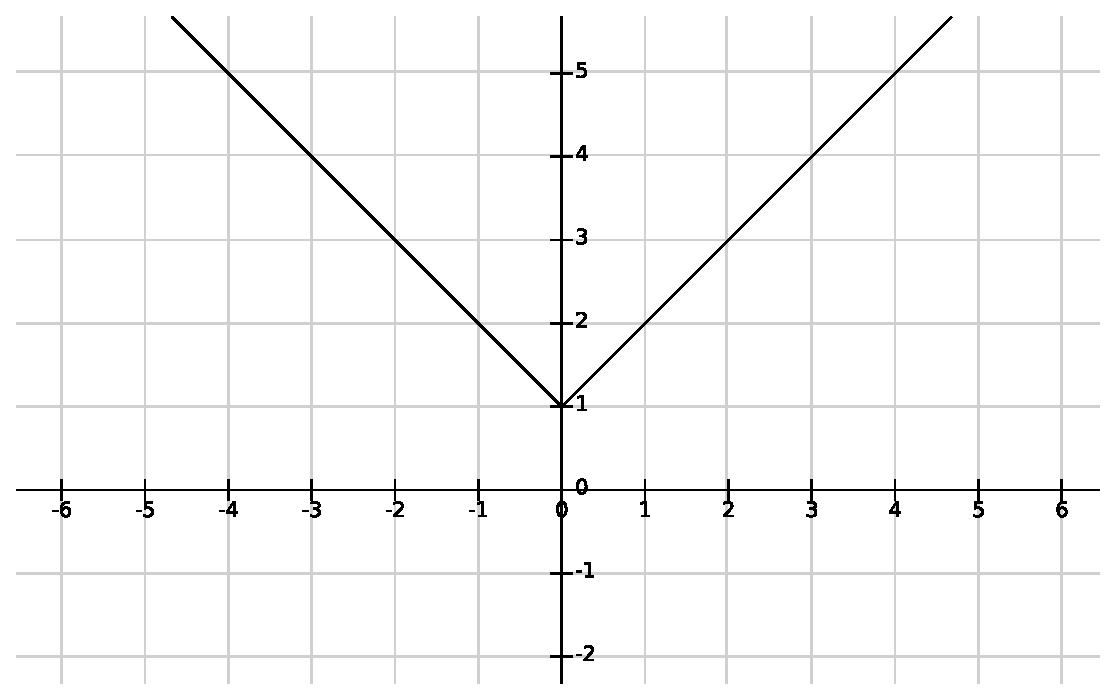
\includegraphics[scale=0.6]{figure_1}

\item $y=|x+3|$ \\

Adding $3$ to $x$ shifts the graph \textit{left} by $3$: \\

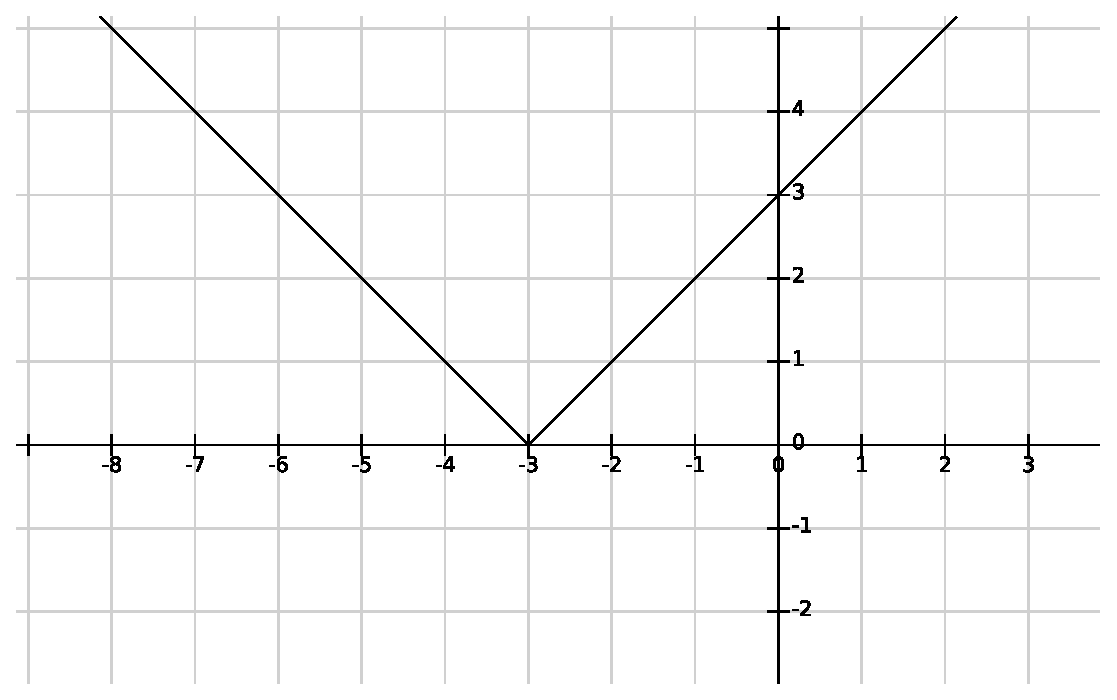
\includegraphics[scale=0.6]{figure_2}

\item $y=3-|x+1|$ \\

Adding $1$ to $x$ shifts the graph \textit{left} by $1$. 
The minus sign flips the graph vertically. 
Then the graph is moved \textit{up} by $3$.
So the graph finally looks like this: \\

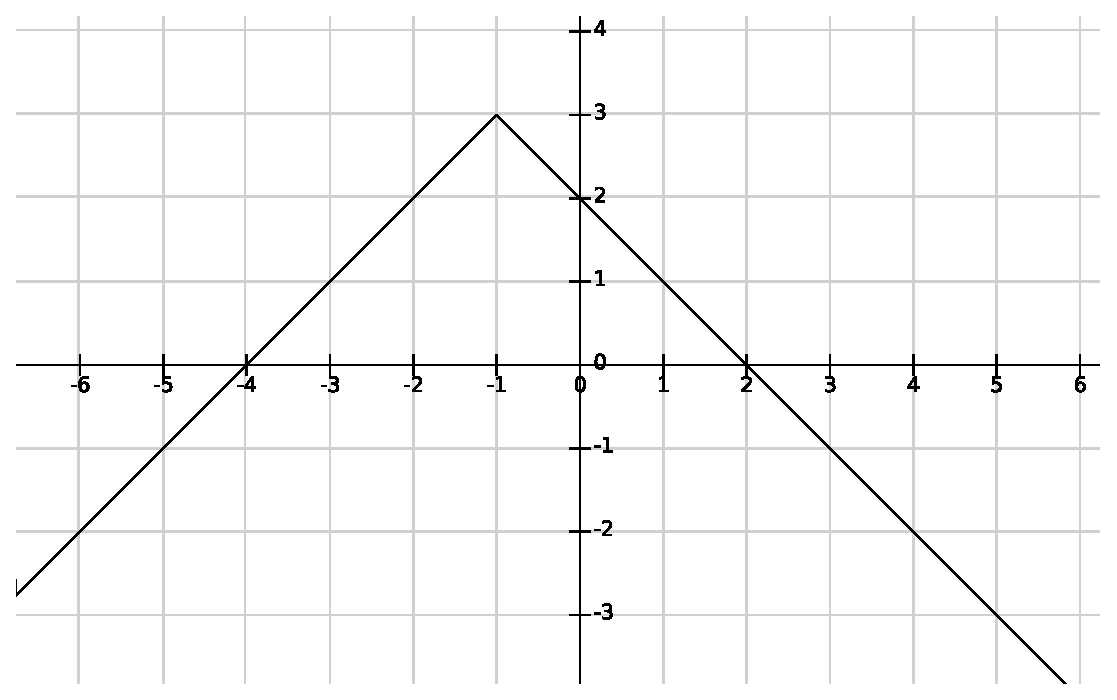
\includegraphics[scale=0.6]{figure_3}

\end{enumerate}


%---------------------%
\subsection*{PROBLEM 2}

If $f(x) = x^3 - 2$ and $g(x) = (1 - x)x^2$, compute:

\begin{enumerate}[label=(\alph*)]

\item $f + g$ 

$$ f+g = x^3-2 + (1-x)x^2 = x^3-2+x^2-x^3 = x^2-2 $$

\item $f - g$

$$ f-g = x^3-2 - (1-x)x^2 = x^3-2-x^2+x^3 = 2x^3-x^2-2 $$

\item $fg$

$$ fg = (x^3-2)(1-x)x^2 = (x^3-2)(x^2-x^3) = -x^6+x^5+2x^3-2x^2 $$

\item $\dfrac{f}{g}$

$$ \dfrac{f}{g} = \dfrac{x^3-2}{(1-x)x^2} = \dfrac{x^3-2}{x^2-x^3},\ 
x \neq 0\ \textrm{and}\ x \neq 1 $$

\item $f(g(1))$

$$ f(g(1)) = f((1-1) \cdot 1^2) = f(0) = 0^3-2 = -2 $$

\item $g(f(1))$

$$ g(f(1)) = g(1^3-2) = g(-1) = (1+1)(-1)^2 = 2 $$

\end{enumerate}


%---------------------%
\subsection*{PROBLEM 7}

The following functions are strictly increasing in their domains. Find the domains of their inverses, and formulas for the inverses.

\begin{enumerate}[label=(\alph*)]

\item $f(x) = 3 + \ln{(e^x - 2)}$, $x > \ln{2}$ \\

$x>\ln{2}$ implies $e^x-2>0$. $\ln{(e^x - 2)}$ takes up the whole range of $\mathbb{R}$. 

Therefore, the range of $f(x)$ is $\mathbb{R}$. \\

Since the domain of $f^{-1}$ is the range of $f$, the domain of $f^{-1}$ is $\mathbb{R}$. \\

Let $y = f(x) = 3 + \ln{(e^x - 2)}$, solve for $x$:

\begin{equation*}
\begin{aligned}
y = 3 + \ln{(e^x - 2)} &\iff
y - 3 = \ln{(e^x - 2)} \\ &\iff
e^{y - 3} = e^x - 2 \\ &\iff
e^x = e^{y - 3} + 2 \\ &\iff
x = \ln{(e^{y - 3} + 2)}
\end{aligned}
\end{equation*}

Therefore, the formulas of the inverse is:

$$ f^{-1}(x) = \ln{(e^{x - 3} + 2)} $$ 

\item $f(x) = \dfrac{a}{e^{-\lambda x} + a}$, $a$ and $\lambda$ positive, $x \in (-\infty, \infty)$ \\

Given that $f(x)$ is strictly increasing. $f(x)$ approaches its minimal as $x$ approaches $-\infty$. $f(x)$ approaches its maximal as $x$ approaches $\infty$. \\

As $x \to -\infty$, $e^{-\lambda x} \to \infty$, which drives $f(x)$ to $0$.

As $x \to \infty$, $e^{-\lambda x} \to 0$, which drives $f(x)$ to $1$. \\

Therefore, the range of $f$ is $(0,1)$, which is also the domain of $f^{-1}$. \\

To get the formula of the inverse function, let $y = f(x)$, solve for $x$:

\begin{equation*}
\begin{aligned}
y = \frac{a}{e^{-\lambda x} + a} &\iff
e^{-\lambda x} + a = \frac{a}{y} \\ &\iff
e^{-\lambda x} = \frac{a}{y} - a \\ &\iff
-\lambda x = \ln{(\frac{a}{y} - a)} \\ &\iff
x = -\frac{1}{\lambda}\ln{(\frac{a}{y} - a)}
\end{aligned}
\end{equation*}

Therefore,

$$ f^{-1}(x) = -\frac{1}{\lambda}\ln{(\frac{a}{x} - a)} $$

\end{enumerate}


%---------------------%
\subsection*{PROBLEM 8}

Determine the distance between the following pairs of points:

\begin{enumerate}[label=(\alph*)]

\item $(2,3)$ and $(5,5)$

$$ d = \sqrt{(2-5)^2 + (3-5)^2} = \sqrt{3^2 + 2^2} = \sqrt{9 + 4} = \sqrt{13} $$

\item $(-4,4)$ and $(-3,8)$

$$ d = \sqrt{(-4+3)^2 + (4-8)^2} = \sqrt{1^2 + 4^2} = \sqrt{1 + 16} = \sqrt{17} $$

\item $(2a,3b)$ and $(2-a,3b)$

$$ d = \sqrt{(2a-2+a)^2 + (3b-3b)^2} = \sqrt{(3a-2)^2} = |3a-2| $$

\end{enumerate}


%---------------------%
\subsection*{PROBLEM 10}

A point $P$ moves in the plane so that it is always equidistant from each of the points $A=(3,2)$ and $B=(5,-4)$. Find a simple equation that the coordinates $(x, y)$ of $P$ must satisfy. \\

The distance from $P$ to $A$ is: $$ d_1 = \sqrt{(x-3)^2 + (y-2)^2} $$

The distance from $P$ to $B$ is: $$ d_2 = \sqrt{(x-5)^2 + (y+4)^2} $$

By definition, we have:

$$ \sqrt{(x-3)^2 + (y-2)^2} = \sqrt{(x-5)^2 + (y+4)^2} $$

Square both side of the equation:

$$ (x-3)^2 + (y-2)^2 = (x-5)^2 + (y+4)^2 $$

Simplify the equation, we get finally:

$$ x - 3y = 7 $$

which is the equation $(x,y)$ must satisfy.

\end{document}